\section{System Model}
\label{s:model}
Our system comprises normal users communicating through autoencoder wireless systems and covert users aiming to establish hidden communication without arousing suspicion. Communication between normal users can be single-user (i.e., a single transmitter and receiver) or multi-user (i.e., multiple transmitters and a base station receiver). First, we describe the system model in the single-user case, simplifying the system by eliminating interference complexity. This applies to systems handling user interference at higher levels or using multiple access techniques like Orthogonal Frequency Division Multiple Access (OFDMA), Code Division Multiple Access (CDMA), and Time Division Multiple Access (TDMA) \cite{WALRAND2000305}. Next, we continue with a more complex scenario, which is the multi-user case with interfering signal transmissions. Our single-user and multi-user system models are illustrated in Figs. \ref{fig:system_architecture} and \ref{fig:multi_system_architecture}, respectively.
\begin{figure*}[thp]
	\center
	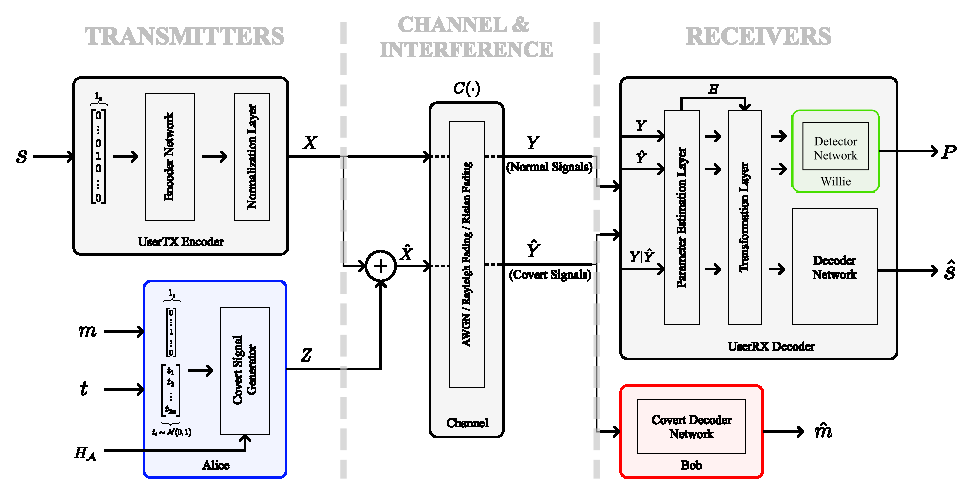
\includegraphics[width=.7\linewidth]{figs/system_architecture}
	\caption{Overall architecture of our system model in the single-user scenario. The UserTX uses an encoder network to encode a binary message $s$ into a vector of signals $X$. Alice generates a covert signal vector $Z$ for a covert message $m$. Willie receives both normal $Y$ and covert $\hat{Y}$ signals during training, but at the time of operation, performs covert detection on either signal based on covert user activity. Similarly, UserRX extracts the normal messages from either $Y$ or $\hat{Y}$. Bob decodes the covert message from $\hat{Y}$. The colored components are accessible to covert users, while the gray components are inaccessible.}	
	\label{fig:system_architecture}
\end{figure*}

\subsection{Single-User Communication}
\textbf{Transmitter}: In the single-user case, the encoder or the transmitter is referred to as UserTX, and the decoder or the receiver is referred to as UserRX. These two entities together form our autoencoder-based normal wireless communication system. The normal communication process begins with UserTX encoding a binary message to a vector of signals using its encoder network. This vector of signals is then transmitted to UserRX and gets distorted while passing through the channel.

\textbf{Channel}: We consider three channel models of AWGN, Rayleigh fading, and Rician fading. To set the \textit{Signal to Noise Ratio} (SNR) in the AWGN model, we keep the transmitter's average power at unit power and adjust the noise power accordingly. For the fading channels, we consider a flat-frequency block-fading channel model, where each signal vector (codeword) is assumed to be faded independently.

\textbf{Receiver}: A noisy version of the transmitted signal is received at the receiver side, where UserRX extracts the message by decoding the signals. In the case of fading channels, the receiver equalizes the signals before passing them to the decoder network.

\textbf{Equalization}: The channel matrix is estimated by UserRX using a blind channel estimation technique, by feeding the received signals to a preliminary network to predict the fading coefficients. Using the estimated channel matrix, UserRX equalizes the signals prior to feeding them to the decoder network. In Fig. \ref{fig:system_architecture} under the \textit{RECEIVERS} section, you can see the two layers of ``Paramter Estimation Layer'' and ``Transformation Layer'' that are responsible for the signal equalization process.

\subsection{Multi-User Communication}
\textbf{Transmitter}: In the multi-user case, multiple transmitters (UserTXs) communicate with a single base station (BaseRX), which serves as the central receiver. Each UserTX uses its own encoder network to encode a binary message to a vector of signals. The transmitters have no knowledge of each other's messages and share no parameters in their networks. Each UserTX and BaseRX pair forms an autoencoder model, with UserTX serving as the encoder and BaseRX as the decoder. After encoding their messages into signals, the transmitters simultaneously send their signals over the channel.

\textbf{Channel}: The multi-user case has the same channel models as described in the single-user case, with the exception that signals experience interference due to simultaneous transmission.

\textbf{Receiver}: BaseRX receives the signals from all the transmitters using multiple antennas after they pass through the channel. It decodes the messages in the same way as the UserRX in the single-user case, but it handles the decoding process for all the transmitters' signals.

\textbf{Equalization}: Similar to the single-user case, BaseRX equalizes the signals before passing them to the decoder networks. However, unlike the single-user receiver, we assume that BaseRX has access to the channel matrix. In practice, BaseRX can use a pilot-based channel estimation technique, which results in a much more accurate estimation of the channel matrix compared to the blind channel estimation used in the single-user case.

\begin{figure*}[thp]
	\center
	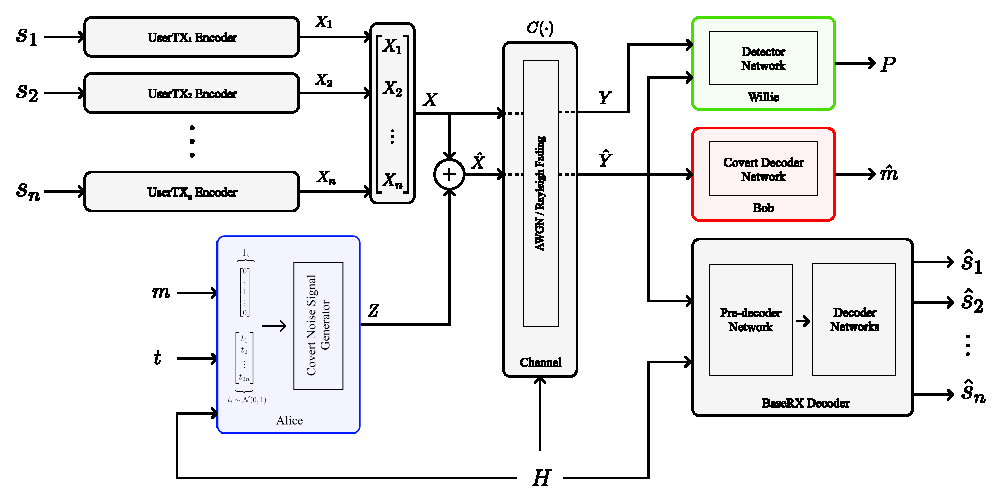
\includegraphics[width=.7\linewidth]{figs/multi_system_architecture}
	\caption{The overall architecture of our system model in the multi-user scenario. Each UserTX separately encodes binary messages $s_i$s into individual signal vectors denoted as $X_i$ ($X$ is a vector of these vectors). Alice generates a covert signal vector $Z$ for a covert message $m$. Willie receives both normal $Y$ and covert $\hat{Y}$ signals during training, but at the time of operation, performs covert detection on either signal based on covert user activity. Similarly, UserRX extracts the normal messages from either $Y$ or $\hat{Y}$. Bob decodes the covert message from $\hat{Y}$. The colored components are accessible to covert users, while the gray components are inaccessible.}
	\label{fig:multi_system_architecture}
\end{figure*}

\subsection{Covert Communication}
There is a covert sender (Alice) who wants to communicate secretly with her intended receiver (Bob). Bob's existence is no secret to the other entities in the system and anyone, including the observer (Willie), can see his transmissions. However, when Willie suspects that a covert sender like Alice is communicating with Bob, he becomes alerted. Therefore, the primary goal of our covert users is to maintain Alice's communications covert.

\textbf{Alice}: The covert communication starts with Alice using her generative model to embed a confidential message into a covert signal vector. You can find an overview of Alice's network in Figs. \ref{fig:system_architecture} and \ref{fig:multi_system_architecture} under the \textit{TRANSMITTERS} sections. As illustrated in the plots, in non-fading channels, Alice merely needs a covert message and a random trigger to produce a covert signal. However, in fading channels, she requires the channel state information of her channel to Bob in the single-user case, and also the channel state information from other normal users to Bob in the multi-user case. This information will be provided by Bob, which we will explain below. After Alice produces the covert signals, she transmits them into the shared channel irrespective of other users' transmissions. This means that her covert signals should be agnostic to the signals of the normal users.

\textbf{Bob}: Unlike the normal receiver or Willie, Bob uses a single antenna at his receiver. He receives the covert signals that have undergone channel effects and interference from normal users' transmissions. Without any equalization operation, he uses his decoder network to extract Alice's message from the covert signals. Additionally, he provides Alice with his and other users' channel information. He does first by sending pilot signals to Alice, and second by measuring channel information using the pilot signals sent from normal transmitters to BaseRX and then broadcasting it to Alice. Bob's existence need not be hidden and him broadcasting this information or pilot signals poses no risk to Alice's secrecy, who is supposed to remain covert.

\textbf{Willie}: Willie listens to all ongoing transmissions on the channel and uses a binary classifier network to determine the likelihood of each signal being covert or normal. Any distortion in the normal signals can alert Willie to the presence of a covert transmission, so Alice must carefully select her covert signals. This means she should not make noticeable changes to the statistical properties of the channel noise or other normal signals. The covert signals should also not increase the system's error rate, as an unexpected increase in the error rate can raise suspicion. We consider Willie to be an integrated module at the receiver of the normal communication system, i.e., UserRX in the single-user and BaseRX in the multi-user case. This way, he can not only detect incoming covert signals but also measure the communication's error rate.

We represent the roles of Alice, Bob, and Willie with DNNs in a training setup similar to GANs. In this adversarial training setting, each of the three roles is encouraged to maximize its performance until they all reach a state of equilibrium at the end of training.

\section{GAN-Based Covert Design}
\label{s:gan_covert}
For a given binary secret message \(m\), Alice first applies a one-hot encoding technique, and then utilizes her generator model to produce a covert signal \(Z\). With this stochastic generative model, each time a different covert signal is generated for the same message. Alice then sends this covert signal to the shared channel, which is accessible to all entities within the system. To simplify notations, we use \(\hat{X}\) to denote the covert signal before propagation.

\begin{equation}
	\hat{X} = X + Z.
\end{equation}

We consider three channel models: AWGN, Rayleigh fading, and Rician fading. Therefore, there will be three different channel outputs for these three channel models. We use a mapping function \(\mathcal{C}(\cdot)\) to express each of these channels' outputs. Since signals in the multi-user case also experience interference, we express single-user and multi-user channel's outputs separately.

\textit{AWGN Channel Output}: For the AWGN channel model, the signal received at the receiver carries the channel's noise effect \(N \sim \mathcal{N}(0, \sigma^2)\). Consequently, the channel function \(\mathcal{C}(\cdot)\) and the final covert signal \(\hat{Y}\) in the single-user case can be represented as:
\begin{equation}
	\hat{Y} = \mathcal{C}(\hat{X}) = X + Z + N.
\end{equation}
For the multi-user case the covert signal can be denoted as:
\begin{equation}
	\hat{Y} = \mathcal{C}(\hat{X}) = \sum_{i \in U}X_i + Z + N.
\end{equation}
where \(U\) is the set that contains all transmitters.

\textit{Rayleigh and Rician Fading Channel Outputs}: In Rayleigh and Rician fading channels, transmitted signals are multiplied by a complex Gaussian random variable with zero mean and a certain variance, which represents the fading effect caused by multipath propagation. Let \(H_{\mathcal{U}}\) be the complex fading coefficient(s) for the normal signal vector(s), and \(H_{\mathcal{A}}\) be the complex fading coefficient for Alice's signal. The channel function \(\mathcal{C}(\cdot)\) and the resulting covert signal \(\hat{Y}\) in the single-user case are given by:
\begin{equation}
	\hat{Y} = \mathcal{C}(\hat{X}) = (H_{\mathcal{U}} \cdot X) + (H_{\mathcal{A}} \cdot Z) + N.
\end{equation}

In the multi-user case, the received covert signal including the channel interference can be written as:
\begin{equation}
	\hat{Y} = \mathcal{C}(\hat{X}) = \sum_{i \in U}(H_{\mathcal{U}_i} \cdot X_i) + (H_{\mathcal{A}} \cdot Z) + N.
\end{equation}

On the receiving end, Bob receives the covert signal \(\hat{Y}\) and uses his decoder network to reconstruct the covert message \(\hat{m}\).

Willie's network is designed to classify sequences of normal signals \(Y\) and covert signals \(\hat{Y}\). In order to ensure that the covert signals remain indistinguishable, Alice must generate them in such a way that Willie's network classifies them as normal signals. To achieve this, Alice requires access to the classifier used by Willie's network. However, this is not feasible in a real-world scenario. Therefore, Alice and Bob perform a black-box attack against Willie's network using a substitute binary classifier. Previous studies have shown that adversarial attacks against one model can be effective on another model, even if the two models have different training sets and architectures \cite{papernot2016transferability}. Willie's substitute network will be used to provide feedback to Alice during training, helping her modify the produced covert signals to make them indistinguishable from normally transmitted signals. This ensures that when the model is deployed in a real communication setup, it is highly unlikely that any observer will detect the covert transmissions.

\subsection{General Formulation}
\textbf{Reliability}: The first objective of our covert model is to enable reliable covert communication. In order to achieve this, Bob needs to be able to accurately decode the covert messages sent by Alice. As mentioned earlier, Alice employs a generative model to produce covert signals that correspond to the covert message. Let \(\Theta_{\mathcal{A}}(\cdot)\) be the underlying function of Alice's generative model that takes a random trigger \(t \sim \mathcal{N}(0, 1)\), a covert message \(m\), the channel coefficients from Alice to Bob \(H_{\mathcal{A}}\), and in the multi-user case, the channel matrix \(H_{\mathcal{U}}\) and produces a covert signal \(Z\). The corresponding covert signal can be denoted as \(Z_{m, t} = \Theta_{\mathcal{A}}(m, t, H_{\mathcal{A}}\footnotemark[1], H_{\mathcal{U}}\footnotemark[2])\). Let  \(\Theta_{\mathcal{B}}(\cdot)\) be the underlying function of the decoder network that Bob uses to reconstruct the covert message \(\hat{m}\). Then the reliability of communication between Alice and Bob is achieved using the following loss function:
\begin{equation}
	\begin{aligned} \label{bob_loss}
		\mathcal{L}_{\mathcal{B}} & = \mathbb{E}_{m}[\mathcal{H}(\hat{m}, m)] \\
		& = \mathbb{E}_{m}[\mathcal{H}(\Theta_{\mathcal{B}}(\hat{Y}), m)] \\ 
		& = \mathbb{E}_{m}[\mathcal{H}(\Theta_{\mathcal{B}}(\mathcal{C}(\hat{X})), m)] \\ 
		& = \mathbb{E}_{m}[\mathcal{H}(\Theta_{\mathcal{B}}(\mathcal{C}(\Theta_{\mathcal{A}}(m, t, H_{\mathcal{A}}) + X)), m)].
	\end{aligned}
\end{equation}
For the multi-user case, this equation is written as:
\begin{equation}
	\begin{aligned}
		\mathcal{L}_{\mathcal{B}} & = \mathbb{E}_{m}[\mathcal{H}(\hat{m}, m)] \\
		& = \mathbb{E}_{m}[\mathcal{H}(\Theta_{\mathcal{B}}(\mathcal{C}(\Theta_{\mathcal{A}}(m, t, H_{\mathcal{A}}, H_{\mathcal{U}}) + X)), m)].
	\end{aligned}
\end{equation}
The equation above uses the cross-entropy function \(\mathcal{H}(\cdot)\) to measure the difference between the probability distribution of the reconstructed covert message \(\hat{m}\) and that of the actual covert message \(m\). This equation can be used to optimize the networks of both Alice and Bob by freezing one or the other's network parameters iteratively.

\footnotetext[1]{Parameter only used in fading channels.}
\footnotetext[2]{Parameter only used in multi-user fading channels.}

\textbf{Low Interference}: While (\ref{bob_loss}) ensures communication accuracy, we also need to ensure that the generated perturbations do not negatively impact normal communication between UserTX and UserRX. Otherwise, this could alert Willie to abnormal activity. To address this, we add a constraint that minimizes UserRX's loss function during Alice's training. In a single-user system, we can express this constraint as follows:
\begin{equation}
	\begin{aligned} \label{alice_user_loss}
		\mathcal{L}_{\mathcal{U}} & = \mathbb{E}_{m}[\mathcal{H}(\hat{s}, s)] \\
		& = \mathbb{E}_{m}[\mathcal{H}(\Theta_{\mathcal{U}}(\hat{Y}), s)] \\
		& = \mathbb{E}_{m}[\mathcal{H}(\Theta_{\mathcal{U}}(\mathcal{C}(\hat{X})), s)] \\
		& = \mathbb{E}_{m}[\mathcal{H}(\Theta_{\mathcal{U}}(\mathcal{C}(\Theta_{\mathcal{A}}(m, t, H_{\mathcal{A}}) + X)), s)].
	\end{aligned}
\end{equation}
where \(\Theta_{\mathcal{U}}(\cdot)\) refers to UserRX's decoder network function. It is important to note that during this training, UserRX's decoder network is frozen and only Alice's parameters will be updated.

For the multi-user case, since we have multiple transmitters sending signals, we need to minimize BaseRX's loss function over all individual transmitters' signals. Thus, (\ref{alice_user_loss}) is rewritten as follows:
\begin{equation}
	\begin{aligned} \label{multi_alice_user_loss}
		\mathcal{L}_{\mathcal{U}} & = \sum_{i \in U}\mathbb{E}_{m}[\mathcal{H}(\hat{s}_i, s_i)] \\
		= \sum_{i \in U} &
		\mathbb{E}_{m}[\mathcal{H}
		(\Theta_{\mathcal{U}}(\mathcal{C}(\Theta_{\mathcal{A}}(m, t, H_{\mathcal{A}}, H_{\mathcal{U}}) + X),  H_{\mathcal{U}}), s_i)].
	\end{aligned}
\end{equation}

\textbf{Undetectability}: In our model, Willie acts as a critic network, similar to what is known as a discriminator in GAN models \cite{goodfellow2014generative}. The so-called real and fake samples in a GANs' discriminator training process here are mapped to normal and covert signals, respectively. For the single-user case, we use the following loss function to optimize Willie's network that classifies covert and normal signals:
\begin{equation}
	\begin{aligned} \label{willie_loss}
		\mathcal{L}_{\mathcal{W}} & = \mathbb{E}_{m}[\mathcal{H}(\hat{Y}, Y)] \\
		& = \mathbb{E}_{m}[\mathcal{H}(\mathcal{C}(\hat{X}), \mathcal{C}(X))] \\
		& = \mathbb{E}_{m}[\mathcal{H}(\mathcal{C}(\Theta_{\mathcal{A}}(m, t, H_{\mathcal{A}}) + X), \mathcal{C}(X))].
	\end{aligned}
\end{equation}
where \(\mathcal{H}(\cdot)\) is the binary cross entropy between the predicted outputs for the covert signals \(\hat{Y}\) or the normal signals \(Y\) and their actual outputs. For the multi-user case, we need to optimize Willie's network over all the transmitters' outputs.

\begin{equation}
	\begin{aligned} \label{multi_willie_loss}
		\mathcal{L}_{\mathcal{W}} & = 
		\sum_{i \in U} \mathbb{E}_{m}[H(\hat{Y}, Y)] \\
		& = \sum_{i \in U}
		\mathbb{E}_{m}[\mathcal{H}(\mathcal{C}(\Theta_{\mathcal{A}}(m, t, H_{\mathcal{A}}, H_{\mathcal{U}}) + X), \mathcal{C}(X))].
	\end{aligned}
\end{equation}

This white-box adversarial training against Alice's network allows Willie's network to distinguish between covert and normal signals when adequately trained. On the other hand, we also ensure that the covert signals generated by Alice maintain the statistical properties of normal signals on the channel to avoid detection. To achieve this undetectability property, we use Willie's network to act as a discriminator network in Alice's optimization function. Alice's training against this network aims to maximize Willie's uncertainty in his predictions, allowing Alice to form covert communication that resembles channel noise while being intelligible to Bob. Overall, Alice's loss function can be expressed as a weighted sum of these three objectives:
\begin{equation}
	\begin{array}{l} \label{alice_loss}
		\mathcal{L}_{\mathcal{A}} = \lambda_{\mathcal{B}} \mathcal{L}_{\mathcal{B}} + \lambda_{\mathcal{U}} \mathcal{L}_{\mathcal{U}} - \lambda_{\mathcal{W}} \mathcal{L}_{\mathcal{W}}.
	\end{array}
\end{equation}
where \(\lambda_{\mathcal{B}}\), \(\lambda_{\mathcal{U}}\), and \(\lambda_{\mathcal{W}}\) are hyperparameters that determine the relative importance of the different objectives in Alice's loss function. The algorithmic steps involved in training our covert models are summarized in Algorithm \ref{alg:train}.

\begin{algorithm}[tp!]
	\caption{Training covert models algorithm}\label{alg:train}
	\small
	\begin{algorithmic}
		\State $X \gets$ normal signals data
		\State $S, M \gets$ normal and covert messages sets
		\State $\Theta_{\mathcal{A}}, \Theta_{\mathcal{B}}, \Theta_{\mathcal{W}} \gets$ Alice, Bob, and Willie networks
		\State $\Theta_{\mathcal{U}} \gets$ UserRX decoder network
		\State $\mathcal{H} \gets$ cross entropy 
		\State $\mathcal{C} \gets$ channel mapping function
		\For{epoch $ep \in \{1 \ldots n_{epochs}$\}}
		\State $t \sim \mathcal{N}(0, 1)$
		\State $\mathcal{L}_{\mathcal{W}} = \mathcal{H}(\mathcal{C}(X), \mathcal{C}(\Theta_{\mathcal{A}}(M, t, H_{\mathcal{A}}, H_{\mathcal{U}}) + X))$
		\State Update $\Theta_{\mathcal{W}}$ to minimize $\mathcal{L}_{\mathcal{W}}$
		\State $\mathcal{L}_{\mathcal{B}} = \mathcal{H}(\mathcal{C}(\Theta_{\mathcal{A}}(M, t, H_{\mathcal{A}}, H_{\mathcal{U}}) + X), M)$
		\State Update $\Theta_{\mathcal{B}}$ to minimize $\mathcal{L}_{\mathcal{B}}$
		\State $\mathcal{L}_{\mathcal{U}} \gets \mathcal{H}(\Theta_{\mathcal{U}}(\mathcal{C}(\Theta_{\mathcal{A}}(M, t, H_{\mathcal{A}}, H_{\mathcal{U}}) + X)), S)$
		\State
		$\mathcal{L}_{\mathcal{A}} = \lambda_{\mathcal{B}} \mathcal{L}_{\mathcal{B}} + \lambda_{\mathcal{U}} \mathcal{L}_{\mathcal{U}} - \lambda_{\mathcal{W}} \mathcal{L}_{\mathcal{W}}$
		\State Update $\Theta_{\mathcal{A}}$ to minimize $\mathcal{L}_{\mathcal{A}}$
		\EndFor
	\end{algorithmic}
\end{algorithm}


\subsection{Neural Network Architecture}
\textbf{User's Autoencoder Network}: The autoencoder model takes a binary message \(s\) of size \(k\) bits and produces a reconstructed version \(\hat{s}\). The encoder maps the message to a \(2 \times n\) signal vector, where \(n\) is the number of channel uses, using one-hot encoding. In the multi-user case, the resulting vector has a size of \(n_{tx} \times (2 \times n)\). The signals pass through the channel, where the channel mapping function applies its effects. In single-user systems with channel fading, the receiver uses parameter estimation and transformation to equalize signals. A simple transformation function divides signals by the estimated channel fading coefficients. More complex transformations can be used, as described in \cite{o2017introduction}; however optimizing the autoencoder model's performance is beyond the scope of this article. In multi-user systems, the decoder receives channel coefficients, allowing BaseRX to use the zero-forcing technique \cite{garg2010wireless} for signal equalization. In single-user systems, UserRX reconstructs the message using its decoder network. In the multi-user case, BaseRX decodes signals from all transmitters simultaneously by passing them through a pre-decoder network and using separate decoders at the final layers.


\textbf{Alice's Network}: Alice first transforms a covert message \(m\) to its corresponding one-hot encoding representation, where each message belongs to a unique class. She then uses a random trigger \(t\) to randomize the process by which the covert noise signal \(Z\) is produced, along with the channel coefficients \(H_{\mathcal{A}}\) and \(H_{\mathcal{U}}\). For Alice's generator model, we use multiple dense layers with ReLU and Tanh activation functions. The first layer acts as an embedding layer, enlarging the input's domain space. The subsequent fully connected layers extract useful features and perform the encoding process. Finally, the last layer performs a dimension transformation, ensuring that the generated covert signal \(Z\) complies with the dimension of the normal signal \(X\) on the channel. 


\textbf{Bob's Network}: Bob receives the covert signal \(\hat{Y}\) that has been affected by the channel, and he feeds it through his decoder network to extract the secret message. Bob's network is more sophisticated than Alice's, as decoding such a distorted signal is a much more complex task. The received message first goes through a wide dense layer with a Tanh activation function, which increases the input's feature space. The data then passes through multiple 1-Dimensional Convolutional (1D Conv) layers, which learn the coding that Alice has developed to encode the covert messages. We have found that using 1D Conv layers helps Bob and Alice achieve better consistency in the accuracy of their communication, especially when the channel model is more complicated (i.e., when there is also fading in the channel). The rest of Bob's decoder network consists of two dense layers that remap the learned feature space to the covert message domain space. As with UserRX's and BaseRX's decoder networks, Bob eventually predicts the covert message by performing a classification on the received signal.

\textbf{Willie's Network}: Willie's task is to distinguish between the normal signal  \(Y\) and the covert  signal \(\hat{Y}\). To achieve this, he uses a neural network with the same architecture as Bob's, except for the last layer, which has a Sigmoid activation function instead of Softmax. The network takes an input signal, either normal or covert, and produces a confidence probability \(P\) indicating the likelihood of the signal being normal. Using the same network architecture for both Bob and Willie ensures a fair competition between them, as they have the same capacity for learning.

\begin{figure*}[tp!]
	\centering
	\begin{subfigure}{0.28\textwidth}
		\includegraphics[width=\linewidth]{figs/autoencoder_bler_awgn}
		\caption{AWGN channel}
	\end{subfigure}
	\begin{subfigure}{0.28\textwidth}
		\includegraphics[width=\linewidth]{figs/autoencoder_bler_rician}
		\caption{Rician fading channel}	
	\end{subfigure}
	\begin{subfigure}{0.28\textwidth}
		\includegraphics[width=\linewidth]{figs/autoencoder_bler_rayleigh}
		\caption{Rayleigh fading channel}	
	\end{subfigure}
	\caption{Autoencoders' performance in terms of BLER over a range of SNR values is evaluated in our single-user case. The models are trained over AWGN, Rayleigh, and Rician fading channels for a set of parameters that have the same data rate.}
	\label{fig:autoencoder_bler}
\end{figure*}
